\documentclass{article}
\usepackage{graphicx} % Required for inserting images
\usepackage[italian]{babel}
\usepackage{amsmath}
\usepackage[hidelinks]{hyperref}
\usepackage{amssymb}
\usepackage{xcolor}

\newcommand{\defeq}{\overset{\mathrm{def}}{=\joinrel=}}

\newtheorem{theorem}{Teorema}

\title{Calcolo differenziale}
\author{Leonardo Ganzaroli}
\date{}

\begin{document}

\maketitle

\addcontentsline{toc}{section}{\protect\numberline{}Introduzione}

\tableofcontents

\newpage

\hypersetup{allcolors=black}

\section*{Introduzione}

Questi appunti del corso \textit{Calcolo differenziale} sono stati creati durante la laurea Triennale di informatica all'università "La Sapienza".

\newpage

\section{Richiami}

\textbf{Prima di procedere rivedere la parte di insiemistica e funzioni negli appunti di \textit{Metodi Matematici per l'informatica}}.

\subsection{Insiemi numerici}

\textbf{Definizione} L'insieme dei numeri naturali $\mathbf{N}$ è definito dagli assiomi di Peano:
\begin{itemize}
    \item $0\in\mathbf{N}$
    \item $n\in\mathbf{N}\Rightarrow succ(n)\in\mathbf{N}$
    \item $\forall\ n,m\in\mathbf{N}\ \ n\neq m\Rightarrow succ(n)\neq succ(m)$
    \item $\nexists n\in\mathbf{N}\ |\ 0=succ(n)$
    \item $\forall\ S\subseteq\mathbf{N}\ \ (0\in S \ \wedge\ n\in S \Rightarrow succ(n))\Rightarrow S=\mathbf{N}$\newline
\end{itemize}

\noindent\textbf{Definizione} L'insieme dei numeri primi è:
$$\mathbf{P}=\{p\in\mathbf{N}-\{1\}\ |\ \nexists a,b\in\mathbf{N}-\{1,p\}\ |\ p=ab\}$$\newline

\noindent\textbf{Definizione} L'insieme dei numeri interi è:
$$\mathbf{Z}=\mathbf{N}\cup\{-n\ |\ n\in\mathbf{N}\ \}$$\newline

\noindent\textbf{Definizione} L'insieme dei numeri razionali è:
$$\mathbf{Q}=\{(p,q)\ |\ p\in\mathbf{Z},q\in\mathbf{Z}-\{0\}\ \}\ \text{, un numero razionale è rappresentato come }\frac{p}{q}$$\newline

\noindent\textbf{Definizione} L'insieme dei numeri reali ($\mathbf{R}$) è l'insieme di tutti i possibili numeri con sviluppo decimale infinito o meno.\newline

\noindent\textbf{Definizione} L'insieme dei numeri complessi è:
$$\mathbf{C}=\{a+ib\ |\ a,b\in\mathbf{R}\ \}\ \text{ con $i^2=-1$}$$\newline

\subsubsection{Intervalli numerici}

Per poter indicare un intervallo di valori tra 2 elementi di un insieme numerico si possono usare le seguenti notazioni:
\begin{itemize}
    \item \textbf{Intervallo aperto}

    $$(a,b)\defeq \{x\in S\ |\ a<x<b\}$$

    \item \textbf{Intervallo aperto a destra}

    $$[a,b)\defeq \{x\in S\ |\ a\leq x< b\}$$

    \item \textbf{Intervallo aperto a sinistra}

    $$(a,b]\defeq \{x\in S\ |\ a< x\leq b\}$$

    \item \textbf{Intervallo chiuso}

    $$[a,b]\defeq \{x\in S\ |\ a\leq x\leq b\}$$\newline

    
\end{itemize}

\subsubsection{Altre definizioni}

\noindent\textbf{Definizione} Dato $I$ sottoinsieme di un insieme numerico. $I$ è detto denso se $\forall \ a,b\in I\ \ a<b\Rightarrow \exists x\in I\ |\ a<x<b$.\newline

\noindent\textbf{Definizione} Dato $I$ sottoinsieme di un insieme numerico. Il massimo di $I$ è il suo elemento $x$ per cui $\forall\ y\in I\ \ x\geq y$.\newline

\noindent\textbf{Definizione} Dato $I$ sottoinsieme di un insieme numerico. Il minimo di $I$ è il suo elemento $x$ per cui $\forall\ y\in I\ \ x\leq y$.\newline

\noindent\textbf{Definizione} Dato $I$ sottoinsieme di un insieme numerico $S$. Il maggiorante di $I$ è ogni valore $x\in S$ tale che $\forall\ y\in I \ \ y\leq x$.\newline

\noindent\textbf{Definizione} Dato $I$ sottoinsieme di un insieme numerico $S$. Il minorante di $I$ è ogni valore $x\in S$ tale che $\forall\ y\in I \ \ y\geq x$.\newline

\newpage

\noindent Espandendo questi ultimi 2 concetti definisco:
\begin{itemize}
    \item \textbf{Estremo superiore}

    $$sup(I)=min\{\text{maggioranti di I}\}$$

    Si dice che $I$ è limitato superiormente da $sup(I)$, nel caso non esista $sup(I)=+\infty$.

    \item \textbf{Estremo inferiore}

    $$inf(I)=max\{\text{minoranti di I}\}$$

    Si dice che $I$ è limitato inferiormente da $inf(I)$, nel caso non esista $sup(I)=-\infty$.
    
\end{itemize}

\noindent\rule{\textwidth}{0.5pt}\newline

\noindent Dato l'intervallo $(5,+\infty)\subset\mathbf{R}$:
\begin{itemize}
    \item Minimo e massimo non esistono
    \item I minoranti sono i numeri $\leq5$, i maggioranti non esistono
    \item L'estremo inferiore è 5
    \item L'estremo superiore è $+\infty$
\end{itemize}

\noindent\rule{\textwidth}{0.5pt}

\subsection{Polinomi}

\textbf{Definizione} Dato un insieme numerico $S$. Un monomio in $S$ è il prodotto tra una costante $a\in S$ ed una o più potenze $x^\alpha y^\beta\ldots\ $ con $\alpha,\beta,\ldots\geq0$, il valore più grande tra questi ultimi è detto \textit{grado del monomio}.\newline

\noindent\textbf{Definizione} Dato un insieme numerico $S$. Un polinomio in $S$ è una somma di monomi in $S$, il grado del polinomio è il grado più grande tra i monomi.\newline

\noindent In generale si può descrivere un polinomio di grado $n$ con coefficienti $c_1,c_2,\ldots,c_n$ e a singola variabile come:

$$p(x)=c_0+c_1x+c_2x^2+\ldots+c_nx^n$$\newline

\noindent\textbf{Definizione} Le radici di un polinomio sono l'insieme di valori che se sostituiti alle variabili portano il polinomio a valore nullo.\newline

\subsubsection{Operazioni}

\begin{itemize}
    \item \textbf{Somma}

    La somma tra $p(x)=a_0+a_1x+\ldots+a_nx^n$ e $q(x)=b_0+b_1x+\ldots+b_mx^m$ con $m\leq n$:

    $$(a_0+b_0)+(a_1+b_1)x+\ldots+(a_m+b_m)x^m+a_{m+1}x^{m+1}+\ldots
    a_nx^n$$

    Il grado del risultato è il grado massimo tra i 2 polinomi.

    \item \textbf{Prodotto}

    Il prodotto tra i polinomi visti sopra:

    $$a_0b_0+a_0b_1x+a_ob_2x^2+\ldots+a_0b_mx^m+\ldots+a_nb_0x^n+a_nb_1x^{n+1}+a_nb_mx^{n+m}$$

    Il grado del risultato è la somma dei gradi dei 2 polinomi.\newline
    
\end{itemize}

\subsection{Equazioni e disequazioni}

\textbf{Definizione} Un'equazione è una formula che esprime eguaglianza tra 2 espressioni matematiche con variabili simili.\newline

\noindent\rule{\textwidth}{0.5pt}

$\text{Esempio: } 5x+88y-3=3x^3-15y$

\noindent\rule{\textwidth}{0.5pt}\newline

\noindent\textbf{Definizione} La legge di annullamento del prodotto afferma che dato un insieme di termini $x_1,x_2,\ldots,x_n$:

$$x_1*x_2*\ldots*x_n=0\iff \text{ almeno un termine è 0}$$\newline

\noindent\textbf{Definizione} Una disequazione è simile ad un'equazione ma $=$ viene sostituito con $<,>,\leq,\geq$.\newline

\noindent\rule{\textwidth}{0.5pt}

$\text{Esempio: } -6x\leq 15+7x-y$

\noindent\rule{\textwidth}{0.5pt}\newline

\noindent\textbf{Definizione} Il cambio del segno permette di passare ad un'altra disequazione equivalente:

$$x\leq y \rightarrow -x\geq -y$$\newpage

\noindent\textbf{Definizione} La regola dei segni afferma che:

$$xy>0\iff (x,y>0\vee x,y<0)$$\newline

\noindent Combinando quest'ultima con la legge di annullamento si ottiene:

$$xy\geq0\iff (x,y\geq0\vee x,y\leq0)$$\newline

\noindent Di conseguenza:
$$xy<0\iff ((x>0\wedge y<0)\vee(x<0\wedge y>0))$$\newline

\noindent Per usare questo principio in modo più semplice è possibile usare il grafico del segno.\newline

\noindent\textbf{Definizione} Un sistema di equazioni (o disequazioni) è un insieme di equazioni in cui le variabili devono rispettare tutte le equazioni presenti:

\[
\text{Esempio:} 
\begin{cases}
12x*9y=334\\
3x+4y=0 
\end{cases}
\]\newline

\subsection{Funzioni a variabile reale}

\textbf{Definizione} Una funzione a variabile reale è una funzione  $f:S\subseteq\mathbf{R}\rightarrow\mathbf{R}$.\newline

\noindent\textbf{Definizione} Una funzione è ben definita se associa ad ogni elemento del dominio un solo elemento del codominio.\newline

\noindent\textbf{Definizione} Il campo di esistenza di una funzione è il massimo sottoinsieme $S\subseteq\mathbf{R}$ per cui la funzione è ben definita se $S$ è il dominio.\newline

\noindent\textbf{Definizione} Una funzione è pari se $\forall\ x\in\text{ dominio}\ \ f(x)=f(-x)$.\newline

\noindent\textbf{Definizione} Una funzione è dispari se $\forall\ x\in\text{ dominio}\ \ f(x)=-f(-x)$.\newline

\noindent\textbf{Definizione} Una funzione è periodica se $\exists c\ |\ \forall\ x\in\text{ dominio}\ \ f(x)=f(x+c)$.\newline

\noindent\textbf{Definizione} Dato $I$ sottoinsieme del dominio. Una funzione è monotona crescente in $I$ se $\forall\ x_1,x_2\in I\ \ f(x_1)\leq f(x_2)\ \text{ con }x_1<x_2$, se invece $f(x_1)\geq f(x_2)$ è decrescente.

\subsubsection{Segno}

Trovare il segno di una funzione vuol dire trovare gli intervalli del dominio per cui la funzione ha valore maggiore o minore di 0, ci sono 3 passaggi:
\begin{enumerate}
    \item Trovare il campo di esistenza
    \item Trovare i valori per cui $f(x)\geq0$
    \item Trovare l'intersezione tra il campo e i valori trovati al punto precedente
\end{enumerate}

\noindent\rule{\textwidth}{0.5pt}\newline

\noindent Considerando $\frac{x^2-1}{2^x-1}$:

\begin{itemize}
    \item Per evitare lo 0 al denominatore $x$ deve essere diverso da 0, quindi $\mathbf{R}-\{0\}$
    \item Risolvo la disequazione $\geq0$:
    \begin{itemize}
        \item $x^2-1\geq 0\rightarrow x\geq1\vee x\leq-1$
        \item $2^x-1\geq 0\rightarrow x\geq0$
    \end{itemize}
\end{itemize}

\noindent Usando il grafico del segno si ottiene:

\begin{figure}[ht]
    \centering
    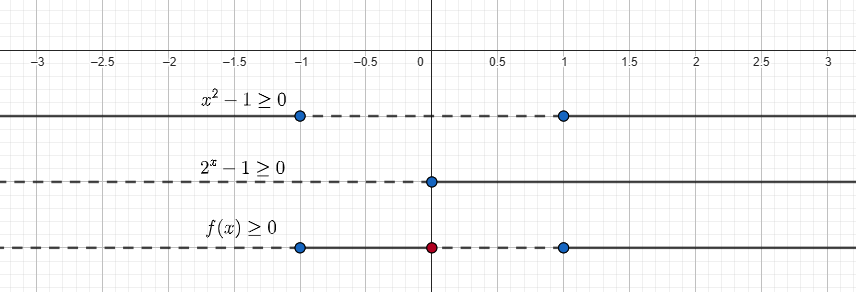
\includegraphics[width=\linewidth]{sign_func.png}
    \label{fig:sign_func}
\end{figure}

\noindent Quindi la funzione è positiva quando $-1\leq x< 0\vee x\geq1$.

\noindent\rule{\textwidth}{0.5pt}

\newpage

\section{Limiti}

\subsection{Punti di accumulazione}

\textbf{Definizione} Dati $x_0,\epsilon\in\mathbf{R}$ con $\epsilon>0$. L'intorno chiuso in $x_0$ di raggio $\epsilon$ ($I_\epsilon[x_0]$) è l'intervallo chiuso $[x_0-\epsilon,x_0+\epsilon]$, analogamente si definisce quello aperto.\newline

\noindent\textbf{Definizione} Dati $I\subseteq\mathbf{R}$ e $x_0\in I$. $x_0$ è:
\begin{itemize}
    \item Punto interno di $I$ se $\ \exists\epsilon>0\ |\ I_\epsilon(x_0)\subset I$
    
    \item Punto esterno ad $I$ se $\ \exists\epsilon>0\ |\ I_\epsilon(x_0)\subset I^C$
    
    \item Punto di frontiera di $I$ se $\ \forall\epsilon>0 \ \ \exists a\in I,b\in I^C\ |\ a,b\in I_\epsilon(x_0)$\newline
    
\end{itemize}

\noindent\textbf{Definizione} Dati $I\subset\mathbf{R}$ e $x_0\in \mathbf{R}$. $x_0$ è un punto di accumulazione se:

$$\forall\ \epsilon>0\ \ \exists x\in I-\{x_0\}\ |\ x\in I_\epsilon(x_0)$$\newline

\subsection{Limite di funzione}

\textbf{Definizione} Il limite di una funzione in un punto di accumulazione esprime la quantità a cui tende il valore della stessa avvicinandosi a quel punto, data la funzione $f:I\rightarrow\mathbf{R}$ e $x_o\in I$ si dice:
\begin{itemize}
    \item \textbf{Convergenza}
    \begin{itemize}
        \item \textbf{$x_0$}

        $f$ converge al valore $l$ ($\lim_{x\rightarrow x_0}f(x)=l$) se:
        
        $$\forall\ \epsilon>0\ \ \exists\delta>0\ |\ \forall\ x\in I\ \ \ 0<|x-x_0|<\delta\Rightarrow|f(x)-l|<\epsilon$$

        \item \textbf{$+\infty$}

        $f$ converge al valore $l$ ($\lim_{x\rightarrow +\infty}f(x)=l$) se:
        
        $$\forall\ \epsilon>0 \ \ \exists N>0\ |\ \forall\ x\in I\ \ \ x>N\Rightarrow |f(x)-l|<\epsilon$$

        \item \textbf{$-\infty$}

        $f$ converge al valore $l$ ($\lim_{x\rightarrow -\infty}f(x)=l$) se:
        
        $$\forall\ \epsilon>0 \ \ \exists N>0\ |\ \forall\ x\in I\ \ \ x<-N\Rightarrow |f(x)-l|<\epsilon$$\newline
        
    \end{itemize}

    \item \textbf{Divergenza}
    \begin{itemize}
        \item \textbf{$x_0,+\infty$}

        $f$ diverge positivamente ($\lim_{x\rightarrow x_0}f(x)=+\infty$) se:
        
        $$\forall\ N>0\ \ \exists\delta>0\ |\ \forall\ x\in I\ \ \ 0<|x-x_0|<\delta\Rightarrow f(x)>N$$

        \item \textbf{$x_0,-\infty$}

        $f$ diverge negativamente ($\lim_{x\rightarrow x_0}f(x)=-\infty$) se:

        $$\forall\ N>0\ \ \exists\delta>0\ |\ \forall\ x\in I\ \ \ 0<|x-x_0|<\delta\Rightarrow f(x)<-N$$

        \item \textbf{$+\infty,+\infty$}

        $f$ diverge positivamente ($\lim_{x\rightarrow +\infty}f(x)=+\infty$) se:

        $$\forall\ N>0 \ \ \exists S>0\ |\ \forall\ x\in I\ \ \ x>S\Rightarrow f(x)>N$$\newline

    \end{itemize}

\end{itemize}

\noindent\textbf{Definizione} Una funzione $f$ si dice infinito per $x\rightarrow*$ se:

$$\lim_{x\rightarrow*}f(x)=\pm\infty$$

\noindent Si dice invece infinitesimo se il limite è uguale a 0.\newline

\noindent\textbf{Definizione} In alcuni casi è necessario trovare il limite del punto $x_0$ facendo una distinzione tra quello ottenuto arrivando da sinistra e quello da destra, in questo caso si individuano il limite sinistro ($x\rightarrow x_0^-$) e destro ($x\rightarrow x_0^+$).\newline

\begin{theorem}[Unicità del limite]
    Non possono esistere 2 limiti distinti in un punto di accumulazione:
    $$\lim_{x\rightarrow *}f(x)=l,\lim_{x\rightarrow *}f(x)=m\Rightarrow l=m$$\newline
\end{theorem}

\begin{theorem}[Cambio di variabile]
Dati i 2 limiti $\lim_{x\rightarrow *}f(x)=l,\lim_{y\rightarrow l}g(y)=m$ si ha:

$$\lim_{x\rightarrow *}g(f(x))=\lim_{y\rightarrow l}g(y)=m$$\newline

\end{theorem}

\begin{theorem}[Teorema del confronto]
Dati $f,g,h:I\rightarrow\mathbf{R}$ e $x_0\in I$. Se $\exists\delta>0\ |\ \forall\ x\in I_\delta(x_0)\ \ \ g(x)\leq f(x)\leq h(x)$ si ha:

$$\lim_{x\rightarrow x_0}g(x)=\lim_{x\rightarrow x_0}h(x)=l\Rightarrow\lim_{x\rightarrow x_0}f(x)=l$$\newline

\end{theorem}

\noindent\textbf{Definizione} Due funzioni $f,g$ si dicono simili per $x\rightarrow*$ se:

$$\lim_{x\rightarrow*}\frac{f(x)}{g(x)}=1$$\newline

\subsection{Asintoti}

\textbf{Definizione} Un asintoto verticale di $f$ è una retta $x=x_0$ tale che:

$$\lim_{x\rightarrow x_o^\pm}f(x)=\pm\infty$$\newline

\noindent\textbf{Definizione} Un asintoto orizzontale di $f$ è una retta $y=l$ tale che:

$$\lim_{x\rightarrow \pm\infty}f(x)=\pm l$$\newline

\noindent\textbf{Definizione} Un asintoto obliquo di $f$ è una retta $mx+q$ tale che:

$$\lim_{x\rightarrow \pm\infty}f(x)-(mx+q)=0$$\newline

\subsection{Continuità}

\textbf{Definizione} Una funzione è detta continua se:

$$\forall\ x_0 \text{ punto di accumulazione }\lim_{x\rightarrow x_0}f(x)=f(x_0)$$\newline

\newpage

\noindent Dalla definizione precedente derivano 3 possibili tipi di discontinuità (limiti sullo stesso punto):
\begin{enumerate}
    \item \textbf{Prima specie}

    I limiti SX/DX sono finiti ma diversi.

    \item \textbf{Seconda specie}

    Almeno un limite SX/DX non esiste o diverge.

    \item \textbf{Terza specie}

    Entrambi i limiti sono finiti e uguali ma il valore $f(x_0)$ non coincide con essi.
    
\end{enumerate}

\begin{theorem}[Permanenza del segno]
    Data una funzione continua $f$ e $x_0$ suo punto di accumulazione:
    \begin{itemize}
        \item $f(x_0)>0\Rightarrow \exists\delta>0\ |\ \forall\ x\in I_\delta(x_0)\ \ f(x)>0$
        \item $f(x_0)<0\Rightarrow \exists\delta>0\ |\ \forall\ x\in I_\delta(x_0)\ \ f(x)<0$\newline
    \end{itemize}
\end{theorem}

\begin{theorem}[Esistenza degli zeri]
    Data una funzione continua $f:I\rightarrow\mathbf{R}$ e $a,b\in I$:

$$((f(a)<0\wedge f(b)>0)\vee(f(a)>0\wedge f(b)<0)\Rightarrow\exists c\in[a,b]\ |\ f(c)=0$$\newline
    
\end{theorem}

\begin{theorem}[Valori intermedi]
    Data una funzione continua $f:I\rightarrow\mathbf{R}$ e $[a,b]\subseteq I$:

$$\forall\ x\in[f(a),f(b)]\ \ \exists y\in [a,b]\ |\ x=f(y)$$\newline
    
\end{theorem}

\begin{theorem}[Weierstrass]
    Data una funzione continua $f:I\rightarrow\mathbf{R}$ e $[a,b]\subseteq I$:

$$\exists x_{min},x_{max}\in[a,b]\ |\ \forall\ x\in[a,b]\ \ f(x_{min})\leq f(x)\leq f(x_{max})$$

\noindent Con $x_{min},x_{max}$ detti minimo/massimo relativo.\newline
    
\end{theorem}

\subsection{Successioni numeriche}

\textbf{Definizione} Una successione numerica è una sequenza di valori generata da un pattern.\newline

\noindent Data una successione numerica $a_n:\mathbf{N}\rightarrow\mathbf{R}$, essa è:
\begin{itemize}
    \item Limitata superiormente se $\exists M\geq0\ |\ \forall n\in\mathbf{N}\ \ a_n\leq M$
    
    \item Limitata inferiormente se $\exists M\geq0\ |\ \forall n\in\mathbf{N}\ \ a_n\geq M$
    
    \item Limitata se $\exists M\geq0\ |\ \forall n\in\mathbf{N}\ \  |a_n|\leq M$

    \item Crescente se $\forall n\in\mathbf{N}\ \  a_n\leq a_{n+1}$, strettamente se $<$

    \item Decrescente se $\forall n\in\mathbf{N}\ \  a_n\geq a_{n+1}$, strettamente se $>$\newline

\end{itemize}

\noindent\textbf{Definizione} Date 2 successioni $a_n:n\rightarrow a(n),b_k:k\rightarrow b(k)$. Si definisce sottosuccessione di $a_n$ su $b_k$ la composizione:

$$a_{b_k}:k\rightarrow a(b(k))$$\newline

\noindent Essendo le successioni una restrizione delle funzioni valgono i concetti visti fin'ora riguardo i limiti (chiamati limiti di successione).\newline

\begin{theorem}[Bolzano-Weierstrass]
    Se una successione è limitata esiste almeno una sottosuccessione convergente per $k\rightarrow+\infty$.\newline
\end{theorem}

\begin{theorem}[Limiti di sottosuccessioni]
$$\lim_{n\rightarrow+\infty}a_n=l\Rightarrow\lim_{k\rightarrow+\infty}a_{b_k}=l$$\newline
\end{theorem}

\begin{theorem}[Teorema ponte]

Dati $f:I\rightarrow\mathbf{R}$, $x_0\in I$ punto di accumulazione, $a_n$ successione. Vale:

$$\lim_{x\rightarrow x_0}f(x)=l\text{ (o }\pm\infty)$$

sse:

$$\forall\ a_n\ |\ a_n\rightarrow x_0\text{ (quando }n\rightarrow+\infty)$$

vale anche:

$$
  \lim_{n\rightarrow+\infty}f(a_n)=l\text{ (o }\pm\infty)$$\newline
\end{theorem}

\section{Derivate}

\subsection{Derivate di funzione}

\textbf{Definizione} Dati 2 punti $a(x_0,f(x_0)),b(x_1,f(x_1))$. La retta tra i punti è data dalla formula:

$$r(x)=f(x_0)+\textcolor{blue}{\frac{f(x_1)-f(x_0)}{x_1-x_0}}(x-x_0)$$

\noindent Con la parte \textcolor{blue}{blu} detta rapporto incrementale.\newline

\noindent\textbf{Definizione} Dati $f:I\rightarrow\mathbf{R}$, $x_0\in I$. $f$ è derivabile in $x_0$ se esiste il limite finito $\lim_{h\rightarrow0}\frac{f(x_0+h)-f(x_0)}{h}$, inoltre si definisce derivata di $f$ in $I$:

$$f'(x)\defeq\lim_{h\rightarrow0}\frac{f(x+h)-f(x)}{h}$$\newline

\noindent La derivata permette di misurare la crescita/decrescita di una certa funzione spostandosi di pochissimo dal punto considerato, nel caso di funzioni reali essa corrisponde alla retta tangente della funzione nel punto considerato.\newline

\noindent

\noindent\textbf{Definizione} Dati $f:I\rightarrow\mathbf{R}$, $[a,b]\subseteq I$ e $x_1,x_2\in[a,b]$. $f$ si dice:
\begin{itemize}
    \item Convessa in $[a,b]$ se $\forall\ x\in[a,b]\ \ f(x)\geq f(x_1)+\frac{f(x_2)-f(x_1)}{x_2-x_1}(x-x_1)$

    \item Concava in $[a,b]$ se $\forall\ x\in[a,b]\ \ f(x)\leq f(x_1)+\frac{f(x_2)-f(x_1)}{x_2-x_1}(x-x_1)$\newline
\end{itemize}

\noindent Dati $f:[a,b]\rightarrow\mathbf{R}$ e $x_0\in I$. $x_0$ è:
\begin{itemize}
    \item Punto di massimo relativo di $f$ se $\exists\delta>0\ |\ \forall x\in I_\delta(x_0)\cap[a,b]\ \ f(x)\leq f(x_0)$
    
    \item Punto di minimo relativo di $f$ se $\exists\delta>0\ |\ \forall x\in I_\delta(x_0)\cap[a,b]\ \ f(x)\geq f(x_0)$

    \item Punto di massimo assoluto di $f$ se $\forall x\in[a,b]\ \ f(x)\leq f(x_0)$

    \item Punto di minimo assoluto di $f$ se $\forall x\in[a,b]\ \ f(x)\geq f(x_0)$

    \item Punto critico di $f$ se $f'(x_0)=0$

    \item Punto di flesso se $\ \exists(a,x_0),(x_0,b)\subseteq[a,b]\ |\ \text{ in $(a,x_0)\ f$ è concava e in $(x_0,b)$ è convessa (o viceversa)}$\newline
    
\end{itemize}

\noindent Trovando il segno di una derivata posso trovare 2 caratteristiche della funzione:
    \begin{itemize}
        \item Derivata prima $\rightarrow$ Quando il segno è positivo la funzione cresce
        \item Derivata seconda $\rightarrow$ Quando il segno è positivo la funzione è convessa
    \end{itemize}

\newpage

\subsection{Teoremi}

\begin{theorem}[Derivabilità e continuità]
    Se $f:I\rightarrow\mathbf{R}$ è derivabile in $I$ allora è continua in $I$.\newline
\end{theorem}

\begin{theorem}[Fermat]
    Se $x_0$ è massimo/minimo di $f$ e $f$ è derivabile in $x_0$ allora $f'(x_0)=0$.\newline
\end{theorem}

\begin{theorem}[Rolle]
    Se $f:[a,b]\rightarrow\mathbf{R}$ è continua e derivabile in $(a,b)$ allora $f(a)=f(b)\Rightarrow\exists c\in (a,b)\ |\ f'(c)=0$.\newline
\end{theorem}

\begin{theorem}[Lagrange]
    Se $f:[a,b]\rightarrow\mathbf{R}$ è continua e derivabile in $(a,b)$ allora $\exists c\in (a,b)\ |\ f'(c)=\frac{f(b)-f(a)}{b-a}$.\newline
\end{theorem}

\begin{theorem}[Criterio differenziale di monotonia]
    Se $f:[a,b]\rightarrow\mathbf{R}$ è continua e derivabile in $(a,b)$, $\forall x\in(a,b)$ si ha:
    \begin{itemize}
        \item $f'(x)\geq0\iff f\text{ è monotona crescente in }[a,b]$
        \item $f'(x)\leq0\iff f\text{ è monotona decrescente in }[a,b]$\newline
    \end{itemize}
    
\end{theorem}

\subsection{Polinomio di Taylor}

\textbf{Definizione} Dati $f:[a,b]\rightarrow\mathbf{R}$ e $x_o\in(a,b)$. Il polinomio di Taylor di ordine $n$ di $f$ centrato in $x_0$ ($T_n(f,x_0)$) è definito come:

$$\sum_{n=0}^{\infty}\frac{f^{(n)}(x_0)}{n!}(x-x_0)^n$$\newline

\noindent Con questo polinomio è possibile approssimare una funzione scrivendola come una serie di termini calcolati partendo dalle derivate della funzione stessa in un punto.\newline

\begin{theorem}[Taylor]
    Dati $f:[a,b]\rightarrow\mathbf{R}$ e $x_o\in(a,b)$. Esiste sempre una funzione $R_n(x)$ detta resto infinitesimale per cui:

    $$f(x)=T_n(x;x_0)+R_n(x;x_0)$$
    
\end{theorem}

\newpage

\section{Studio di funzione}

Avendo visto le caratteristiche principali di una funzione è ora possibile analizzarla, bisogna trovare:
\begin{enumerate}
    \item \textbf{Campo di esistenza}
    \item \textbf{Parità}
    \item \textbf{Zeri}
    \item \textbf{Segno}
    \item \textbf{Asintoti}
    \item \textbf{Monotonia}
    \item \textbf{Convessità}
    \item \textbf{Minimi/massimi relativi}
    \item \textbf{Punti di flesso}\newline
\end{enumerate}

\noindent Trovando queste caratteristiche è anche possibile rappresentare la funzione sul piano.\newline

\subsection{Esempio}

\noindent\rule{\textwidth}{0.5pt}\newline

\noindent Studio di $\frac{2x}{x^2-1}$:

\begin{enumerate}
    \item Il campo è $\mathbf{R}-\{1,-1\}$
    \item La funzione è dispari
    \item L'unico zero è $x=0$
    \item La funzione è positiva quando $x>1\vee -1<x\leq0$
    \item Facendo i limiti per $\pm\infty,\pm1$ trovo:
    \begin{itemize}
        \item 2 asintoti orizzontali convergenti a 0 con $\pm\infty$
        \item 2 asintoti verticali divergenti (dx) a $+\infty$ con $\pm1$
        \item 2 asintoti verticali divergenti (sx) a $-\infty$ con $\pm1$
    \end{itemize}

    \newpage
    
    \item Studiando il segno della derivata prima scopro che la funzione è sempre decrescente

    \begin{figure}[ht]
        \centering
        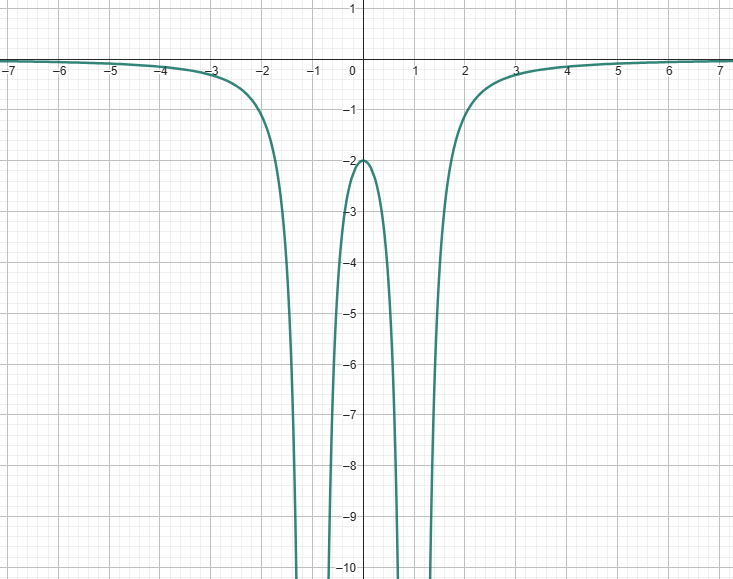
\includegraphics[width=0.575\linewidth]{der1.png}
        \caption{Derivata prima}
        \label{fig:der1}
    \end{figure}
    
    \item Studiando il segno della derivata seconda scopro che la funzione è convessa tra -1,0 e dopo 1

    \begin{figure}[ht]
        \centering
        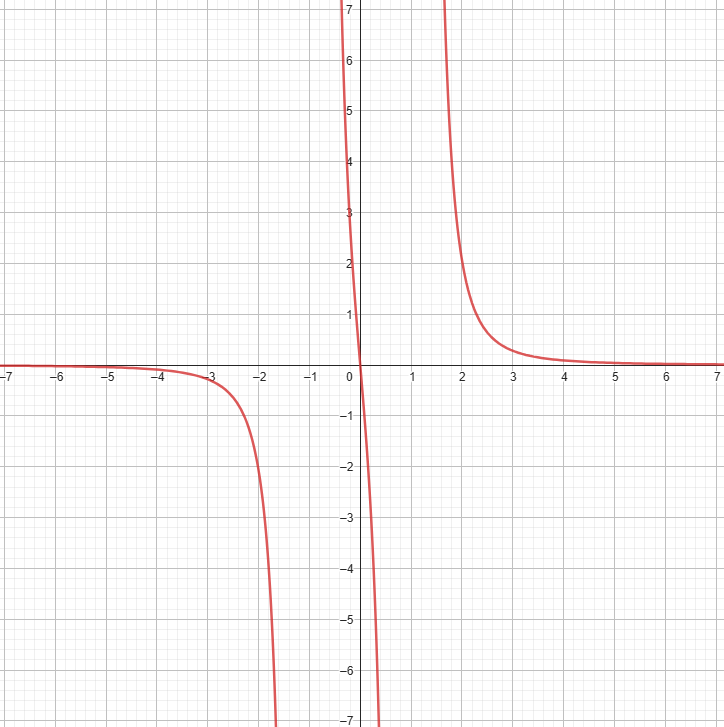
\includegraphics[width=0.575\linewidth]{der2.png}
        \caption{Derivata seconda}
        \label{fig:der2}
    \end{figure}
    
    \item Considerando il punto precedente (0,0) è l'unico punto di flesso\newpage
\end{enumerate}

\noindent Avendo adesso tutte le informazioni si può disegnare il grafico:

    \begin{figure}[ht]
        \centering
        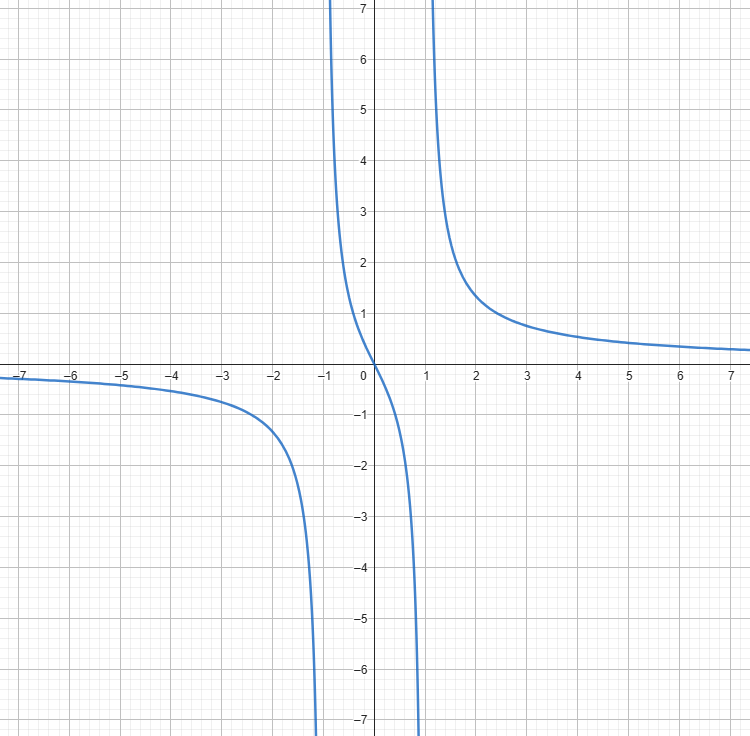
\includegraphics[width=\linewidth]{func.png}
        \caption{$\frac{2x}{x^2-1}$}
        \label{fig:func}
    \end{figure}

\noindent\rule{\textwidth}{0.5pt}\newline

\end{document}
